\chapter{Criterios de optimización y ordenamiento para \textit{piecewise maps} ordenados}

En este capítulo se describen en detalle los distintos \textbf{criterios de optimización} y \textbf{ordenamiento} utilizados en las operaciones sobre \textit{piecewise maps} ordenados. Ambos conjuntos de criterios serán aplicados con el propósito de mejorar la eficiencia general de dichas operaciones y reducir significativamente los tiempos de ejecución.

\textbf{Pseudocódigo y notación:} En este capítulo, al igual que se hizo para los \textit{piecewise maps} desordenados, se emplearán subíndices para referirse a los mapas de un \textit{piecewise map} ordenado con ele fin de alivianar la notación. Dado un \textit{piecewise map} ordenado $A$, el elemento ubicado en la posición $i$, lo cual corresponde a \texttt{pieces\_[i].first} en C++, se denotará como \textbf{$A_i$}, donde $i$ es un número natural que satisface $0 \leq i < |A|$, siendo $|A|$ la cantidad de mapas de $A$.

\section{Operaciones estructuralmente similares}

Como se puede ver en la sección de conceptos previos correspondiente a los \textit{piecewise maps} desordenados, existen muchas operaciones que presentan una estructura muy similar a la de la intersección entre conjuntos desordenados. Entre estas operaciones se encuentran: la \textbf{igualdad}, la \textbf{suma}, la i\textbf{gualdad de imágenes}, la \textbf{resta} y el \textbf{mínimo adyacente}.

Todas estas operaciones, junto con la intersección de conjuntos ordenados, comparten una estructura común que se puede dividir en dos partes: 
\begin{enumerate}
    \item Una\textbf{ fase de comparación}, donde cada elemento de uno de los argumentos es comparado con todos los del otro argumento.
    \item Un \textbf{núcleo de la operación}, donde se ejecuta la lógica específica de la operación sobre aquellos pares de elementos cuya comparación fue satisfactoria.
\end{enumerate}

Esta estructura puede observarse gráficamente en el pseudocódigo presentado en ~\ref{alg:operaciones-simil}.

En el caso de la intersección de conjuntos desordenados, la comparación consiste en verificar si la intersección entre dos multi-intervalos, uno de cada conjunto, es vacía, y el núcleo de la operación se encarga de guardar dicha intersección en el conjunto resultante.

En cambio, para las otras operaciones mencionadas, la comparación consiste en verificar si la intersección entre los dominios de dos mapas, uno de cada \textit{piecewise map} desordenado argumento, es no vacía. El núcleo depende de la operación específica: por ejemplo, en el caso de la suma, se calcula la suma de los mapas y se almacena el resultado en el \textit{piecewise map} desordenado de salida.


\begin{algorithm}
\caption{Estructura de las operaciones similares a la intersección de conjuntos desordenados}\label{alg:operaciones-simil}
\begin{algorithmic}[1]
\Require $A$, $B$ son conjuntos desordenados o dos \textit{piecewise maps} desordenados
\Function{operación}{$A, B$}

\State ... \Comment{Casos base y definiciones necesarias de la operación}

\ForAll{$a \in A$} \Comment{Fase de comparación de la operación.}
    \ForAll{$b \in B$}
        \State $I$ \Comment{Elemento a comparar proveniente de una o varias operaciones entre los elementos $a$ y $b$}
        \If{$\Call{isEmpty}{I}$}
            \State ...  \Comment{Núcleo de la operación.}
        \EndIf
    \EndFor
\EndFor

\State \Return ...
\EndFunction
\end{algorithmic}
\end{algorithm}

Por lo tanto, dado que las operaciones sobre \textit{piecewise maps} desordenados mencionadas anteriormente comparten esta misma estructura, y considerando todas las definiciones introducidas para los \textit{piecewise maps} ordenados, es posible adaptar los criterios de optimización desarrollados para la intersección de conjuntos ordenados a las operaciones mencionadas.

\subsection{Criterios de optimización}

\begin{center}
    \fbox{
        \parbox{0.92\linewidth}{
            \centering
            \textbf{Criterio de parada} \\[1ex]
            \raggedright
            Sean $A$ y $B$ dos \textit{piecewise maps} ordenados. Supóngase que se está evaluando una de las operaciones mencionadas entre ambos, y en particular se consideran los posibles cálculos del núcleo de la operación entre mapa $A_i$ de $A$, con $0 \leq i < |A|$, y los mapas de $B$. Dado un índice $k$ tal que $0 \leq k < |B|$, vale lo siguiente:

            \vspace{0,5cm}
     
            \textbf{Si} el máximo perimetral del dominio de $A_i$ es estrictamente menor que el mínimo perimetral del dominio de $B_k$ en la primera dimensión, \textbf{entonces}:

            \begin{itemize}
                \item la intersección entre el dominio de $A_i$ y el de $B_{k'}$ resulta vacía \textbf{y} no se calcula el núcleo de la operación para $A_i$ y $B_{k'}$, $\forall k' \mid k \leq k' < |B|$;
                \item \textbf{y, entonces,} puede continuarse directamente con la fase de comparación entre $A_{i+1}$(si existe) y los mapas de $B$ para validar el calculo del núcleo de la operación.
            \end{itemize}
    
        }
    }
\end{center}



\begin{center}
    \fbox{
        \parbox{0.92\linewidth}{
            \centering
            \textbf{Criterio de eliminación} \\[1ex]
            \raggedright
            Sean $A$ y $B$ dos \textit{piecewise maps} ordenados. Supóngase que se está evaluando una de las operaciones mencionadas entre ambos, y en particular se consideran los posibles cálculos del núcleo de la operación entre mapa $A_i$ de $A$, con $0 \leq i < |A|$, y los mapas de $B$. Dado un índice $k$ tal que $0 \leq k < |B|$, vale lo siguiente:

            \vspace{0,5cm}
     
            \textbf{Si} el máximo perimetral del dominio de $(B_{k}$ es estrictamente menor que al mínimo perimetral del conjunto $A_{i}$ en la primera dimensión, \textbf{entonces}:

            \begin{itemize}
                \item la intersección entre $A_{i'}$ y $B_{k}$ resulta vacía \textbf{y} no se calcula el núcleo de la operación para $A_{i'}$ y $B_{k}$, $\forall i' \mid i \leq i' < |A|$;
                
                \item \textbf{y, entonces,} puede descartarse $B_k$ para las fases de comparación de los mapas posteriores a $A_i$ y así descartar completamente el calculo del núcleo de la operación $B_k$ con estos.
            \end{itemize}
                
    
        }
    }
\end{center}



\begin{center}
    \fbox{
        \parbox{0.9\linewidth}{
            \centering
            \textbf{Criterio de selección} \\[1ex]
            \raggedright
            Sean dos piecewise maps ordenados involucrados en alguna de las operaciones mencionadas. Se establece lo siguiente:

            \begin{center}
            \textit{
                Se define como $B$ a aquel piecewise map que contiene la menor cantidad de mapas,
                mientras que se denota como $A$ al piecewise map restante.
            }
            \end{center}
        }
    }
\end{center}


\begin{center}
    \fbox{
        \parbox{0.93\linewidth}{
            \centering
            \textbf{Criterio de solapamiento} \\[1ex]
            \raggedright
            Sean $A$ y $B$ dos \textit{piecewise maps}, $A_i$ un mapa de $A$ y $B_k$ uno de $B$, con índices tales que:
            \[
            0 \leq i < |A|, \quad 0 \leq k < |B|.
            \]
            Se establece entonces que, en el caso de realizar una de las operaciones entre $A$ y $B$, y querer calcular el núcleo de la operación entre $A_i$ y 
            $B_k$:

            \begin{itemize}
                \item \textbf{Si} existe solapamiento entre los conjuntos dominio de $A_i$ y $B_k$, \textbf{entonces}:
                \begin{itemize}
                    \item \textbf{Si} ambos conjuntos son \textit{densos}, la intersección entre ellos es necesariamente no vacía y se puede proceder con el calculo del núcleo de la operación.
                    \item \textbf{Si} al menos uno de ellos no es denso, la intersección \textit{puede} ser no vacía, pero no se garantiza de modo que se debe proceder de igual manera.
                \end{itemize}

                \item \textbf{Si} \textbf{no} existe solapamiento entre los conjuntos dominio de $A_i$ y $B_k$, \textbf{entonces} la intersección entre ellos es necesariamente vacía, independientemente de si son densos o no, y por ende puede obviarse el calculo del núcleo de la operación.
            \end{itemize}
        }
    }
\end{center}


En este ultimo caso faltaría definir que es el solapamiento entre conjuntos y cuando un conjunto es denso para poder completar el criterio anterior:

        \begin{center}
            Sean $C$ y $D$ dos conjuntos. Entonces se dice que $C$ y $D$ se solapan o están solapados si y solo si los multi-intervalos definidos a través de sus mínimos y máximos perimetrales se solapan bajo la definición de solapamiento de multi-intervalos ya vista.
        \end{center}

        \begin{figure}[h]
    \centering
    \begin{subfigure}[b]{0.48\linewidth}
        \centering
        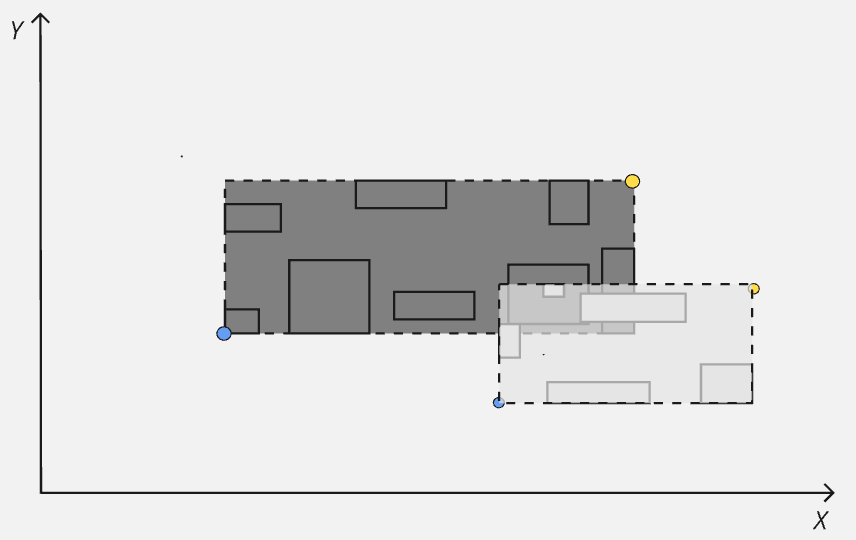
\includegraphics[width=\linewidth]{figures/optimizaciones pwmap/op simils/mi1.png}
        \caption{Conjuntos con sus multi-intervalos definidos con sus máximos y mínimos perimetrales.}
        \label{fig:crit-suma-dominio}
    \end{subfigure}
    \hfill
    \begin{subfigure}[b]{0.48\linewidth}
        \centering
        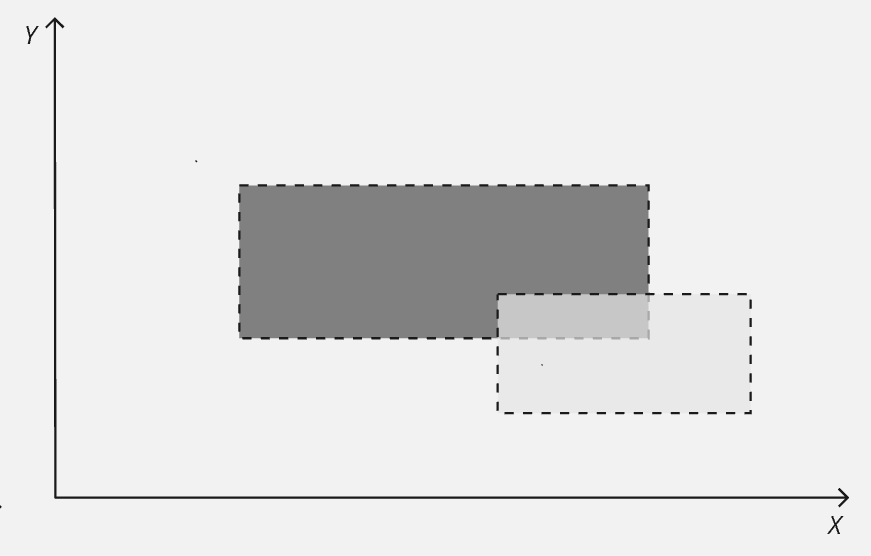
\includegraphics[width=\linewidth]{figures/optimizaciones pwmap/op simils/mi2.png}
        \caption{Solapamiento entre los multi-intervalos definidos.}
        \label{fig:crit-suma-extremos}
    \end{subfigure}
    \caption{Criterios de solapamiento para \textit{piecewise maps} ordenados.}
    \label{fig:crit-suma}
\end{figure}

        \begin{center}
            Sea $C$ el conjunto, y sean $minPer_C$ y $maxPer_C$ el mínimo y máximo perimetral, respectivamente. Entonces se dice que el conjunto es \textbf{denso} si y solo si, si se define un multi-intervalo denso $m$ donde su mínimo y máximo sean $minPer_C$ y $maxPer_C$ respectivamente, entonces:
                \[
                    \{m\} - C = C - \{m\} = \emptyset
                \]
        \end{center}
\begin{figure}[h]
    \centering
    \begin{subfigure}[b]{0.42\linewidth}
        \centering
        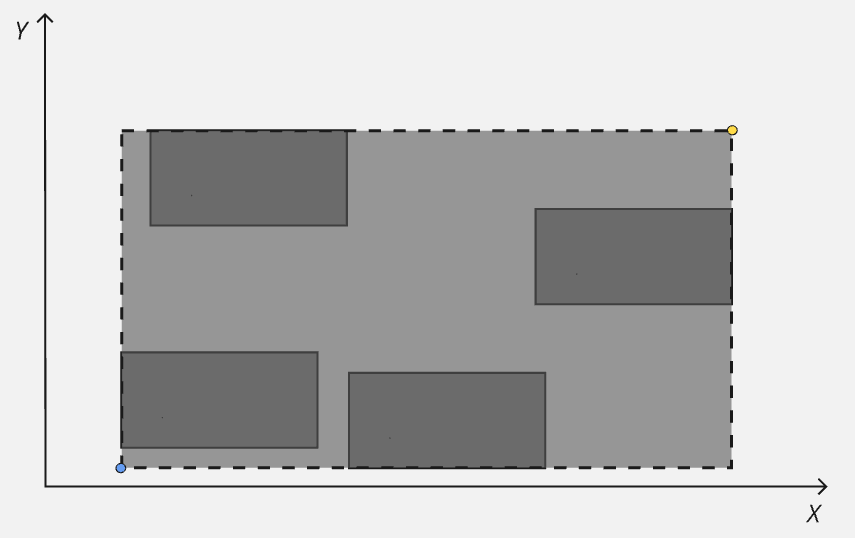
\includegraphics[width=\linewidth]{figures/optimizaciones pwmap/op simils/denso1.png}
        \caption{Conjunto no denso.}
        \label{fig:crit-suma-dominio}
    \end{subfigure}
    \hfill
    \begin{subfigure}[b]{0.42\linewidth}
        \centering
        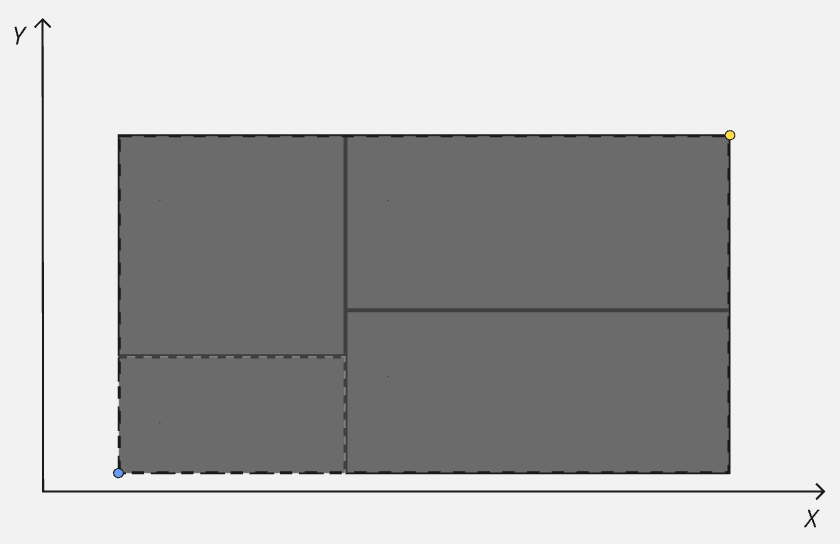
\includegraphics[width=\linewidth]{figures/optimizaciones pwmap/op simils/denso2.png}
        \caption{Conjunto no denso.}
        \label{fig:crit-suma-max}
    \end{subfigure}
    \hfill
    \vspace{0,5cm}
    \begin{subfigure}[b]{0.42\linewidth}
        \centering
        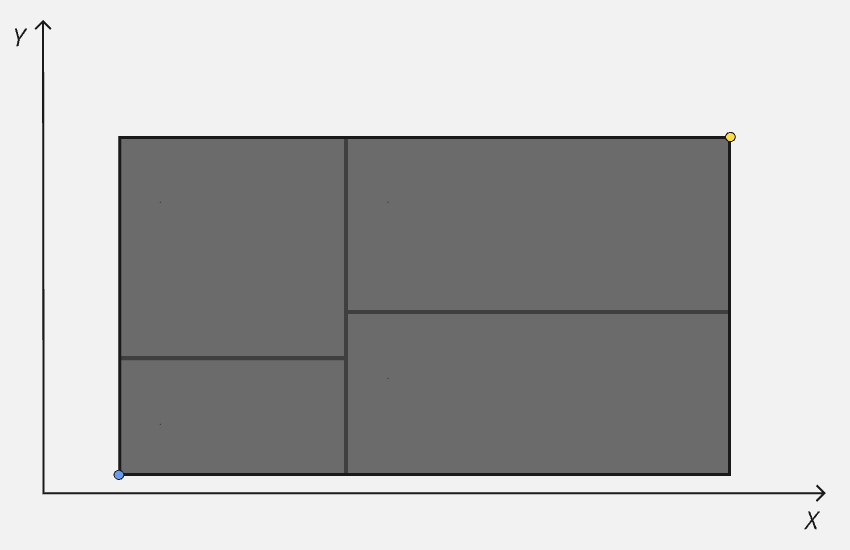
\includegraphics[width=\linewidth]{figures/optimizaciones pwmap/op simils/denso3.png}
        \caption{Conjunto denso.}
        \label{fig:crit-suma-min}
    \end{subfigure}
    \caption{Densidad de conjuntos.}
    \label{fig:crit-suma}
\end{figure}





\subsection{Criterios validos por operación}

Ahora bien, el núcleo de la operación puede variar significativamente dependiendo de la naturaleza de la operación considerada. En consecuencia, el criterio de ordenamiento utilizado también puede diferir considerablemente entre una operación y otra. 

Por esta razón, los criterios específicos serán mencionados y analizados individualmente, operación por operación. 

Además, no todas las operaciones admitirán todos los criterios de optimización previamente definidos. La aplicabilidad de cada criterio dependerá de las particularidades del núcleo de la operación y del comportamiento esperado.


\subsubsection{Igualdad - \texttt{==}}

Para el caso de la igualdad, se pueden aplicar todos los criterios de optimización previamente definidos. 

En cuanto a su \textbf{criterio de ordenamiento}, esta operación no requiere de uno, ya que no produce como resultado un \textit{piecewise map} ordenado. En consecuencia, no dispone de un criterio de ordenamiento asociado.

\subsubsection{suma - \texttt{+}}

En el caso de la suma, vuelven a aplicarse todos los criterios de optimización mencionados. Y, en cuanto a su criterio de ordenamiento, este resulta muy similar al propuesto para la intersección de conjuntos ordenados, con las modificaciones y adaptaciones necesarias claro esta.


\begin{center}
    \fbox{
        \parbox{0.93\linewidth}{
            \centering
            \textbf{Criterio de ordenamiento} \\[1ex]
            \raggedright
            Supóngase que se realiza la suma entre dos \textit{piecewise maps} ordenados, $A$ y $B$, y que se están evaluando las posibles sumas del $i$-ésimo mapa de $A$, denotado por $A_i$, con todos los mapas de $B$. Ademas se cuenta con un \textit{piecewise map} resultado $C$.

            \vspace{1ex}

            Todas las sumas no vacías generadas con $A_i$ deben insertarse en $C$ \textbf{después} de aquellas sumas generadas por los mapas $A_0, A_1, \dots, A_{i-1}$, cuyos mínimos perimetrales sean estrictamente menores al mínimo perimetral de $A_i$, bajo el operador $<$ de naturales multi-dimensionales.
        }
    }
\end{center}


Básicamente es homologo al definido para la intersección de conjuntos ordenados y se fundamenta de la misma manera.

Este criterio se basa nuevamente en la observación de que, al realizar la \textit{suma}, 
su dominio corresponde a la intersección de los dominios de los mapas participantes. 
Dicha intersección entre dos dominios está contenida en ambos, lo que implica que su mínimo perimetral 
se encuentra dentro de los multi-intervalos definidos por el mínimo y el máximo perimetral de los operandos, 
o bien que coincide con el mínimo perimetral de alguno de ellos.  

Al fijar \(A_i\), todas sus sumas posibles con mapas de \(B\) tendran su minimo perimetral dentro del multi-intervalo definido por el mínimo y el máximo perimetral de \(A_i\). 
Como consecuencia, cualquier suma con dominio no vacío generada tendrá un mínimo perimetral mayor o igual 
que el mínimo perimetral de \(A_i\).


Esto garantiza que tales sumas deben insertarse en el \textit{piecewise map} resultado después de aquellas cuyo 
 dominio tenga un mínimo perimetral que sea estrictamente menor al de $A_i$, es decir, las generadas por los mapas anteriores de $A$. Una vez procesado $A_i$, se avanza hacia $A_{i+1}$ y se continúa la construcción del \textit{piecewise map} resultado de la misma manera.

La Figura~\ref{fig:crit-suma} ilustra gráficamente esta situación. Se observa, todas las intersecciones de los dominios de las sumas producidas a partir del mapa $A_i$ con los mapas de $B$. En particular los dominios tienen el mismo nombre que los mapas a los que pertenecen. Y como se ve, estas sumas que realizan la intersección de sus dominios tienen un mínimo perimetral mayor o igual que el del dominio de $A_i$, y se insertan a continuación de los mapas previamente procesadas cuyo mínimo perimetral sea menor al de $A_i$. Esto mismo ocurre con las de $A_{i+1}$ cuya suma con $B_k$ se debe insertar después de los mapas con $A1$ y  $A2$ como dominio.

\begin{figure}[h]
    \centering
    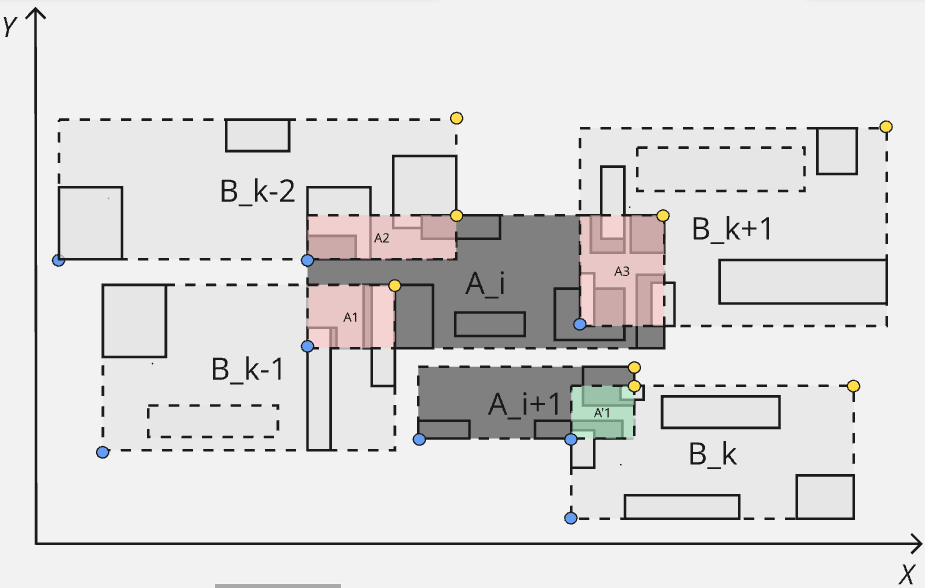
\includegraphics[width=0.8\linewidth]{figures/optimizaciones pwmap/op simils/crit suma.png}
    \caption{Criterio de ordenamiento de la suma para \textit{piecewise map} ordenados de las sumas en función de su dominio y, en particular, de sus mínimos perimetrales.}
    \label{fig:crit-suma}
\end{figure}

Adicionalmente, no es necesario comenzar a verificar la posición de inserción de las sumas en el \textit{piecewise map} resultado desde el principio en cada iteración de los elementos de $A$. Dado el orden intrínseco de los \textit{piecewise map} involucrados, se cumple que
\[
minPer_{i} \leq minPer_{i+1}
\]
 donde $minPer_i$ y $minPer_{i+1}$ son los minimos perimetrales de $A_i$ y $A_{i+1}$ respectivamente.
 
Esto implica que las sumas generadas por $A_{i+1}$ necesariamente deben insertarse a partir de una posición igual o posterior a aquella donde comenzaron a colocarse las sumas de $A_i$ con los elementos de $B$.

Esto desencadena la siguiente modificación del criterio de ordenamiento: 
\begin{center}
    \fbox{
        \parbox{0.93\linewidth}{
            \centering
            \textbf{Criterio de ordenamiento} \\[1ex]
            \raggedright
            Supóngase que se realiza la suma entre dos \textit{piecewise maps} ordenados, $A$ y $B$, y que se están evaluando las posibles sumas del $i$-ésimo mapa de $A$, denotado por $A_i$, con todos los mapas de $B$. Ademas se cuenta con un \textit{piecewise map} resultado $C$.

            \vspace{1ex}

            Todas las sumas no vacías generadas con $A_i$ deben insertarse en $C$ \textbf{después} de aquellas sumas generadas por los mapas $A_0, A_1, \dots, A_{i-1}$, cuyos mínimos perimetrales sean estrictamente menores al mínimo perimetral $A_i$, bajo el operador $<$ de naturales multi-dimensionales.
            
            \vspace{1ex}

            Adicionalmente \textbf{si} la posición a partir de la cual se colocan las sumas de $A_i$ en el \textit{piecewise map} resultante es $k$, con $0 \leq k < |C|$, \textbf{entonces} aquellas generadas por $A_{i+1}$ se insertaran a partir de $k'$ tal que $k \leq k' < |C|$.
        }
    }
\end{center}

\subsubsection{Igualdad de imágenes - \texttt{iqualImage}}

El caso de esta operación es muy similar al de la operación de igualdad: admite todos los criterios de optimización y tampoco requiere un criterio de ordenamiento. Esta última característica, a diferencia del caso de la igualdad, no se debe a que la operación devuelva un valor de verdad, sino a que su resultado es un conjunto en sí mismo, el cual tiene su implementación propia y no se debe alterar.

\subsubsection{Resta - \texttt{-}}

Ahora es el momento de analizar la resta, o el operador \texttt{-}. Esta operación admite todos los criterios de optimización, con excepción del criterio de selección, ya que se trata de una operación donde el orden de los argumentos es relevante y, por lo tanto, no puede alterarse. En cuanto al criterio de ordenamiento, ocurre algo particular.

En el núcleo de la operación desordenada, cuando se calcula la resta entre dos mapas, el proceso genera un resultado parcial únicamente para los dos mapas involucrados. El tamaño de este resultado parcial, o la cantidad de mapas que contiene, depende exclusivamente de la cantidad de dimensiones con las que se esté trabajando. Luego, este resultado parcial se incorpora al \textit{piecewise map} resultado de la operación mediante la operación \texttt{concatenation}.

Ahora bien, con esto presente, el criterio de ordenamiento queda relegado a un esquema muy básico:

\begin{center}
    \fbox{
        \parbox{0.93\linewidth}{
            \centering
            \textbf{Criterio de ordenamiento} \\[1ex]
            \raggedright
            Supóngase que se realiza la resta entre dos \textit{piecewise maps} ordenados, $A$ y $B$. Ademas se cuenta con un \textit{piecewise map} resultado $C$.
            
            \vspace{1ex}
            
            Todos los mapas del resultado parcial obtenido al procesar la resta de un mapa de $A$ y uno de $B$ se ordenan linealmente, salvo que el mapa que se incorpora deba ir al final. Es decir, cada vez que se agrega un mapa al resultado parcial, primero se verifica si este debe colocarse directamente al final; en tal caso, se inserta en esa posición. En caso contrario, se recorren desde el inicio los mapas ya existentes para encontrar su posición, de modo que el resultado parcial se mantenga ordenado.

            \vspace{1ex}
            
            Y, el resultado final, se mantiene ordenado mediante la operación \texttt{concatenation} cada vez que se guarda un resultado parcial.
        }
    }
\end{center}

\subsubsection{Mínimo adyacente - \texttt{minAdjMap}}

Por último, está la operación \texttt{minAdjMap}, la cual puede utilizar todos los criterios de optimización, salvo el de selección, ya que nuevamente el orden de los argumentos tiene relevancia. 

En cuanto al criterio de ordenamiento, aparece un problema que se repite tanto aquí como en varias operaciones sobre \textit{piecewise maps} ordenados: la imagen. La imagen de un mapa, aunque es un conjunto, posee una cohesión que depende tanto del conjunto dominio como de la colección de expresiones lineales del mapa. Por ejemplo, dos mapas pueden tener un mismo dominio, pero basta con que alguna de sus expresiones varíe para que sus imágenes sean distintas. Algo similar ocurre si varía el dominio.

Entonces, ordenar mapas cuyo dominio corresponde a la imagen, o a alguna transformación derivada, de otro mapa perteneciente a un \textit{piecewise map} ordenado resulta una tarea particularmente compleja. En estos casos, el orden del \textit{piecewise map} original aporta escasa o nula información útil para ordenar los mapas derivados, cuyos dominios provienen de dichas imágenes o transformaciones. 

Una alternativa es realizar un ordenamiento estrictamente lineal, lo cual implica un costo computacional elevado, especialmente cuando el \textit{piecewise map} resultante contiene un gran número de mapas.


En conclusión, para poder brindar un orden a un \textit{piecewise map} cuyo contenido son mapas con dominios derivados de imágenes, sería necesario tener en cuenta no solo el dominio, sino también las expresiones y la forma de dichas expresiones. Por esta razón, se concluyó que lo más óptimo es utilizar directamente un algoritmo de ordenamiento, lo cual simplifica el entendimiento de la esta y de las demás operaciones de \textit{piecewise maps} ordenados ya que evita la necesidad de escribir y mantener código de criterios de ordenamiento que, probablemente, tendría un rendimiento inferior.


\section{Restricción de dominio - \texttt{restrict}}

El caso de la operación \texttt{restrict} es diferente al de las operaciones vistas anteriormente. Sin embargo, esto no significa que no puedan adaptarse los criterios definidos previamente para esta operación.

En particular, la operación \texttt{restrict} aplicada a un \textit{piecewise map} desordenado, como ya se vio, consiste en restringir el dominio de cada uno de sus mapas individuales en base a un conjunto, siendo ambos argumentos de la operación, y quedando como parte del resultado solo aquellos mapas del \textit{piecewise map} desordenado cuyos dominios restringidos son no vacíos.

Ahora bien, al dotar de orden al \textit{piecewise map} argumento y requerir que el resultado también esté ordenado, la operación puede beneficiarse de los siguientes criterios de optimización y ordenamiento:

\subsection{Criterios de optimización}


\begin{center}
    \fbox{
        \parbox{0.92\linewidth}{
            \centering
            \textbf{Criterio de parada} \\[1ex]
            \raggedright
            Sean $A$ un \textit{piecewise map} ordenado y $S$ un conjunto. Supóngase que se evalúa la restricción de dominio entre ambos, y en particular se considera la posible restricción de domino del dominio de un mapa $A_i$ de $A$, con $0 \leq i < |A|$, con respecto a $S$. Entonces vale lo siguiente:

            \vspace{0,5cm}
     
            \textbf{Si} el máximo perimetral de $S$ es estrictamente menor que el mínimo perimetral del conjunto dominio de $A_i$ en la primera dimensión, \textbf{entonces}:

            \begin{itemize}
                \item la intersección entre el dominio de $A_i$ y $S$ resulta vacía \textbf{y} no se calcula la restricción de dominio para $A_{i'}$ con respecto a $S$, $\forall i' \mid i \leq i' < |A|$;
                \item \textbf{y, entonces,} puede terminarse directamente con la operación \texttt{restrict}.
            \end{itemize}
    
        }
    }
\end{center}


\begin{center}
    \fbox{
        \parbox{0.93\linewidth}{
            \centering
            \textbf{Criterio de solapamiento} \\[1ex]
            \raggedright
            Sean $A$ un \textit{piecewise map}, $S$ un conjunto y $A_i$ un mapa de $A$ tal que:
            \[
            0 \leq i < |A|.
            \]
            Se establece entonces que, en el caso de realizar la restricción de dominio de $A$ sobre $S$ y querer calcular la restricción de $A_i$ con respecto a $S$:

            \begin{itemize}
                \item \textbf{Si} existe solapamiento entre el conjunto dominio de $A_i$ y $S$, \textbf{entonces}:
                \begin{itemize}
                    \item \textbf{Si} ambos conjuntos son \textit{densos}, la intersección entre ellos es necesariamente no vacía y se puede proceder con el calculo de la restricción del dominio de $A_i$ en base a $S$.
                    \item \textbf{Si} al menos uno de ellos no es denso, la intersección \textit{puede} ser no vacía, pero no se garantiza de modo que se debe proceder de igual manera.
                \end{itemize}

                \item \textbf{Si} \textbf{no} existe solapamiento entre el conjunto dominio de $A_i$ y $S$, \textbf{entonces} la intersección entre ellos es necesariamente vacía, independientemente de si son densos o no, y por ende puede obviarse el calculo de la restricción del dominio de $A_i$ en base a $S$.
            \end{itemize}
        }
    }
\end{center}

\subsection{Criterio de ordenamiento}

En este caso, lo que debe mantenerse ordenado en el \textit{piecewise map} resultante son todas las restricciones de dominio no vacías de los mapas del \textit{piecewise map} ordenado argumento. La restricción de dominio de un mapa consiste únicamente en reemplazar su dominio original por la intersección entre dicho dominio y el conjunto que también llega como argumento.

Ahora bien, como se discutió en el criterio de ordenamiento para la suma, el mínimo perimetral del dominio restringido está contenido dentro de alguno de los multi-intervalos definidos por los máximos y mínimos perimetrales del dominio del mapa a restringir y del conjunto que restringe. Ademas aquí también vale que no es necesario buscar la posición de inserción desde el comienzo del \textit{piecewise map} resultado. Esto permite redefinir el criterio de ordenamiento de la siguiente manera:

\begin{center}
    \fbox{
        \parbox{0.93\linewidth}{
            \centering
            \textbf{Criterio de ordenamiento} \\[1ex]
            \raggedright
            Supóngase que se realiza la restricon de dominio entre un \textit{piecewise map} ordenado $A$ y un conjunto $S$, y que se están evaluando la restricción de dominio del $i$-ésimo mapa de $A$, denotado por $A_i$, con respecto a $S$. Ademas se cuenta con un \textit{piecewise map} resultado $C$.

            \vspace{1ex}

            La restricción no vacía generada con $A_i$ deben insertarse en $C$ \textbf{después} de aquellas restricciones no vacías generadas por los mapas $A_0, A_1, \dots, A_{i-1}$, cuyos mínimos perimetrales sean estrictamente menores al mínimo perimetral de $A_i$, bajo el operador $<$ de naturales multi-dimensionales.

            \vspace{1ex}

            Adicionalmente \textbf{si} la posición a partir de la cual se colocan las sumas de $A_i$ en el \textit{piecewise map} resultante es $k$, con $0 \leq k < |C|$, \textbf{entonces} aquellas generadas por $A_{i+1}$ se insertaran a partir de $k'$ tal que $k \leq k' < |C|$.
        }
    }
\end{center}


\section{Combinación - \texttt{combine}}

El siguiente caso que se analizará es el de la operación \texttt{combine}, una de las ya introducidas previamente en el capítulo de conceptos previos.

Esta operación, como ya se vio, aplicada sobre \textit{piecewise maps} desordenados, toma dos de ellos y realiza una suerte de "unión", devolviendo un único \textit{piecewise map} desordenado. Este contiene todos los mapas del primero, junto con aquellos mapas del segundo cuyos dominios son una reducción, conteniendo ahora solo aquellos valores no presentes en el dominio total del primer \textit{piecewise map}. 

Debido a la naturaleza de su funcionamiento y requerir preservar el orden en el resultado, esta operación emplea únicamente un criterio de optimización y un criterio de ordenamiento, ambos reformulados de los vistos para las \textit{operaciones estructuralmente similares}.

\subsection{Criterio de optimización}

Trabajando con dos \textit{piecewise maps} $A$ y $B$, los únicos mapas de $B$ que pueden formar parte del resultado son aquellos donde la diferencia de su domino con el dominio total de $A$ sea no vacía. El dominio modificado resultante para cada uno de los mapas de $B$ será precisamente dicha diferencia. Por lo tanto, lo único que se puede hacer es omitir la diferencia cuando se sabe que no es necesaria, y de esta observación se deriva el siguiente criterio de solapamiento:

\begin{center}
    \fbox{
        \parbox{0.93\linewidth}{
            \centering
            \textbf{Criterio de solapamiento} \\[1ex]
            \raggedright
            Sean $A$ y $B$ dos \textit{piecewise maps}, $B_k$ un mapa de $B$, tal que:
            \[
            0 \leq k < |B|.
            \]
            y sea $S$ el dominio de $A$. Se establece entonces que, en el caso de realizar la combinación entre $A$ y $B$ y al estar considerando $B_k$ :

            \begin{itemize}
                \item \textbf{Si} existe solapamiento entre el conjunto dominio de $B_k$ y $S$, \textbf{entonces}:
                \begin{itemize}
                    \item \textbf{Si} ambos conjuntos son \textit{densos}, la intersección entre ellos es necesariamente no vacía y se debe proceder con el calculo de la diferencia para obtener el nuevo dominio de $B_k$.
                    \item \textbf{Si} al menos uno de ellos no es denso, la intersección \textit{puede} ser no vacía, pero no se garantiza de modo que se debe proceder de igual manera.
                \end{itemize}

                \item \textbf{Si} \textbf{no} existe solapamiento entre el conjunto dominio de $B_k$ y $S$, \textbf{entonces} la intersección entre ellos es necesariamente vacía, independientemente de si son densos o no, y por ende puede obviarse el calculo de la diferencia,la cual devolvería el mismo dominio de $B_k$, y el dominio de $B_k$ queda intacto.
            \end{itemize}
        }
    }
\end{center}

\subsection{Criterio de ordenamiento}

En cuanto al orden, al realizar la diferencia entre dos conjuntos, por ejemplo, entre dos conjuntos $C$ y $D$, el nuevo mínimo perimetral del conjunto resultante $C - D$ debe encontrarse contenido dentro del multi-intervalo definido por el mínimo y el máximo perimetral del conjunto original $C$. 

Esto se debe a que la operación de diferencia remueve elementos de $C$, sin añadir otros nuevos. Esta observación es casi análoga a lo que ocurría en el caso de la operación de suma, discutido en sección correspondiente a la suma de \textit{piecewise map} ordenados. Análogamente a lo visto tamien en la suma, gracias a lo anterior y al orden de los \textit{piecewise maps}, ocurre que si $B_k$ con su dominio modificado se debería insertar a partir de una posición $i$, con $0 \leq i < |C|$, en el \textit{piecewise map} resultado, entonces $B_k$ con su dominio modificado debería ubicarse en $i'$ tal que $i \leq i' < |C|$

En consecuencia, se postula el siguiente criterio de ordenamiento derivado del visto para el operador \texttt{+}:

\begin{center}
    \fbox{
        \parbox{0.93\linewidth}{
            \centering
            \textbf{Criterio de ordenamiento} \\[1ex]
            \raggedright
            Supóngase que se realiza la combinación entre dos \textit{piecewise maps} ordenados, $A$ y $B$, y que se deba calcular el nuevo dominio para el mapa $k$-ésimo de $B$, denotado por $B_k$, con respecto al dominio de $A$, $S$. Ademas se cuenta con un \textit{piecewise map} resultado $C$.

            \vspace{1ex}

            \textbf{Si} el nuevo dominio de $B_K$ no es vacío, es decir, la resta entre el conjunto dominio de $B_k$ y $S$ es no vacía; \textbf{entonces} el mapa $B_k$ con dominio restringido por $S$ estará ubicado en el \textit{piecewise map} resultante después de todos aquellos mapas cuyo mínimo perimetral sea menor que el minino perimetral del dominio original de $B_k$, bajo el operador $<$ de naturales multi-dimensionales.
            
            \vspace{1ex}

            Adicionalmente \textbf{si} la posición a partir de la cual se coloca de $B_k$ con dominio modificado en el \textit{piecewise map} resultante es $i$, con $0 \leq i < |C|$, \textbf{entonces} el mapa modificado de $B_{k+1}$ se insertaría, si su dominio no es vacio, a partir de $i'$ tal que $i \leq i' < |C|$.
        }
    }
\end{center}


\section{Concatenación - \texttt{concatenation}}

El caso de la operación concatenación, es básicamente homologo al del la unión disjunta de conjuntos, y por ende haciendo las respectivas modificaciones, se puede reutilizar lo visto para la unión disjunta de conjuntos ordenados aquí.

\subsection{Criterio de ordenamiento}

\begin{center}
    \fbox{
        \parbox{0.93\linewidth}{
            \centering
            \textbf{Criterio de ordenamiento}\\[1ex]
            \raggedright
           Sean $A = \{A_0, A_1, \dots, A_{n-1}\}$ y $B = \{B_0, B_1, \dots, B_{m-1}\}$ dos \textit{piecewise maps} no vacíos, disjuntos y ordenados. Sea $C$ un \textit{piecewise map} inicialmente vacío que contendrá el resultado de la fusión ordenada de $A$ y $B$. Y sean $A_i$ un mapa de $A$ y $B_k$ un mapa de $B$, con índices tales que:
            \[
            0 \leq i < |A|, \quad 0 \leq k < |B|.
            \]
            
            \vspace{1ex}

            Entonces, al realizar la unión disjunta entre $A$ y $B$ vale que:

            \begin{itemize}
                \item \textbf{Si} el mínimo perimetral de  $A_i$ es menor, bajo el operador $<$ definido para naturales multi-dimensionales, que el mínimo perimetral de  $B_k$, entonces $A_i$ debe aparecer \textbf{antes} que $B_k$ en el \textit{piecewise map} $C$.
                \item\textbf{Si} el mínimo perimetral de  $A_i$ no es menor, bajo el operador $<$ definido para naturales multi-dimensionales, que el mínimo perimetral de $B_k$, entonces $B_k$ debe aparecer \textbf{antes} que $A_i$ en el \textit{piecewise map} $C$.
            \end{itemize}

            \vspace{1ex}
        }
    }
\end{center}

\section{Desplazamiento de dominio - \texttt{offsetDom}}

Al buscar optimizar y ordenar la salida en la operación \texttt{offsetDom}, cuando esta recibe como argumentos dos \textit{piecewise maps} ordenados, es posible adaptar y reutilizar los criterios previamente establecidos para la operación \texttt{restrict}.

Como se observa en su versión desordenada, para que un mapa de $A$ sea incluido en el resultado, debe existir un desplazamiento no vacío generado por la imagen de $O$ en base al dominio del mapa. Ahora bien, al trabajar con \textit{piecewise maps} ordenados, es posible anticipar si dicho desplazamiento será vacío o no. Para ello, pueden aplicarse criterios de optimización derivados, y adaptados, de aquellos utilizados en la restricción de dominio.

Cabe destacar que, al trabajar con la imagen de un \textit{piecewise map} para generar la salida, 
nuevamente se hará uso de un algoritmo de ordenamiento en lugar de diseñar un criterio de ordenamiento específico, como se hizo para \textit{minAdjMap}.


\subsection{Criterios de optimización}


\begin{center}
    \fbox{
        \parbox{0.92\linewidth}{
            \centering
            \textbf{Criterio de parada} \\[1ex]
            \raggedright
            Sean $A$ y $O$ \textit{piecewise maps} ordenados y $S$ el conjunto dominio de $O$. Supóngase que se evalúa el desplazamiento de dominio entre $A$ y $O$, y en particular se considera el posible desplazamiento de dominio del dominio de un mapa $A_i$ de $A$, con $0 \leq i < |A|$, con respecto a $O$. Entonces vale lo siguiente:

            \vspace{0,5cm}
     
            \textbf{Si} el máximo perimetral de $S$ es estrictamente menor que el mínimo perimetral del conjunto dominio de $A_i$ en la primera dimensión, \textbf{entonces}:

            \begin{itemize}
                \item la intersección entre el dominio de $A_i$ y $S$ resulta vacía \textbf{y} no se calcula el desplazamiento de dominio para $A_{i'}$ con respecto a $S$, $\forall i' \mid i \leq i' < |A|$;
                \item \textbf{y, entonces,} puede terminarse directamente con la operación \texttt{offsetDom}.
            \end{itemize}
    
        }
    }
\end{center}


\begin{center}
    \fbox{
        \parbox{0.93\linewidth}{
            \centering
            \textbf{Criterio de solapamiento} \\[1ex]
            \raggedright
            Sean $A$ y $O$ \textit{piecewise maps} ordenados, $S$ el conjunto dominio de $O$ y $A_i$ un mapa de $A$ tal que:
            \[
            0 \leq i < |A|.
            \]
            Se establece entonces que, en el caso de realizar el desplazamiento de dominio de $A$ en base a $O$, y querer desplazar el dominio de $A_i$ en base a $O$:

            \begin{itemize}
                \item \textbf{Si} existe solapamiento entre el conjunto dominio de $A_i$ y $S$, \textbf{entonces}:
                \begin{itemize}
                    \item \textbf{Si} ambos conjuntos son \textit{densos}, la intersección entre ellos es necesariamente no vacía y se puede proceder con el calculo del desplazamiento de dominio de $A_i$ en base a $O$.
                    \item \textbf{Si} al menos uno de ellos no es denso, la intersección \textit{puede} ser no vacía, pero no se garantiza de modo que se debe proceder de igual manera.
                \end{itemize}

                \item \textbf{Si} \textbf{no} existe solapamiento entre el conjunto dominio de $A_i$ y $S$, \textbf{entonces} la intersección entre ellos es necesariamente vacía, independientemente de si son densos o no, y por ende puede obviarse el calculo del desplazamiento de dominio de $A_i$ en base a $O$.
            \end{itemize}
        }
    }
\end{center}


\section{Composición - \texttt{composition}}

Al intentar optimizar y ordenar el \textit{piecewise map} resultante en la operación \texttt{composition}, cuando esta recibe como argumentos dos \textit{piecewise maps} ordenados, es posible adaptar y reutilizar los criterios previamente establecidos para la operación suma y para las \textit{operaciones estructuralmente similares}.

Como se observa en su versión desordenada optimizada ~\ref{alg:composition-des-opt}, para que el resultado de componer un mapa $A$, $a$, con uno de $B$, $b$, sea incluido en el resultado final, debe tener un dominio no vació. Es decir, la intersección del domino $a$ con la imagen de $b$ debe ser no vacía. Teniendo esto ultimo presente se pueden redefinir los criterios de optimización para las \textit{operaciones estructuralmente similares} y el criterio de ordenamiento que se le dio a la suma. 

\subsection{Criterios de optimización}


\begin{center}
    \fbox{
        \parbox{0.92\linewidth}{
            \centering
            \textbf{Criterio de parada} \\[1ex]
            \raggedright
            Sean $A$ y $B$ dos \textit{piecewise maps} ordenados. Supóngase que se está evaluando la composición entre ambos, y en particular se consideran las posibles composiciones entre un mapa $B_k$ de $B$, con $0 \leq k < |B|$, y los mapas de $A$. Dado un índice $i$ tal que $0 \leq i < |A|$, vale lo siguiente:

            \vspace{0,5cm}
     
            \textbf{Si} el máximo perimetral del dominio de $A_i$ es estrictamente menor que el mínimo perimetral del conjunto imagen de $B_k$ en la primera dimensión, \textbf{entonces}:

            \begin{itemize}
                \item la intersección entre el dominio de $A_{i'}$ y la imagen de $B_{k}$ resulta vacía \textbf{y} no se calcula la composición entre $A_{i'}$ y $B_{k}$, $\forall i' \mid i \leq i' < |A|$;
                \item \textbf{y, entonces,} puede continuarse directamente con verificando las posibles composiciones de $B_{k+1}$(si existe) con los mapas de $A$.
            \end{itemize}
    
        }
    }
\end{center}

\begin{center}
    \fbox{
        \parbox{0.93\linewidth}{
            \centering
            \textbf{Criterio de solapamiento} \\[1ex]
            \raggedright
            Sean $A$ y $B$ dos \textit{piecewise maps}, $A_i$ un mapa de $A$ y $B_k$ uno de $B$, con índices tales que:
            \[
            0 \leq i < |A|, \quad 0 \leq k < |B|.
            \]
            Se establece entonces que, en el caso de realizar la composición entre $A$ y $B$, y querer calcular la composición de $A_i$ y $B_k$:

            \begin{itemize}
                \item \textbf{Si} existe solapamiento entre los conjuntos dominio de $A_i$ e imagen de $B_k$, \textbf{entonces}:
                \begin{itemize}
                    \item \textbf{Si} ambos conjuntos son \textit{densos}, la intersección entre ellos es necesariamente no vacía y se puede proceder con el calculo de la composición entre $A_i$ y $B_k$.
                    \item \textbf{Si} al menos uno de ellos no es denso, la intersección \textit{puede} ser no vacía, pero no se garantiza de modo que se debe proceder de igual manera.
                \end{itemize}

                \item \textbf{Si} \textbf{no} existe solapamiento entre los conjuntos dominio de $A_i$ e imagen de $B_k$, \textbf{entonces} la intersección entre ellos es necesariamente vacía, independientemente de si son densos o no, y por ende puede obviarse el calculo de la composición entre $A_i$ y $B_k$.
            \end{itemize}
        }
    }
\end{center}

\subsection*{Criterio de ordenamiento}

En este caso tenemos que al realizar la composición entre dos mapas, su dominio es un subconjunto del dominio original del primer mapa a componer. Por ende, al fijar el primer mapa, todos sus composiciones no vacías con otros mapas, tendrán un domino con un mínimo perimetral igual o menor que el del dominio del mapa fijado, bajo el operador $<$ de naturales multi-dimensionales. Esto es muy similar a lo que ocurría en la operación \textit{restrict}. Ademas aquí también vale que no es necesario buscar la posición de inserción desde el comienzo del \textit{piecewise map} resultado como se vio para las restricción de dominio.

  
\begin{center}
    \fbox{
        \parbox{0.93\linewidth}{
            \centering
            \textbf{Criterio de ordenamiento} \\[1ex]
            \raggedright
            Supóngase que se realiza la composición entre dos \textit{piecewise maps} ordenados, $A$ y $B$, y que se están evaluando las posibles composiciones del $k$-ésimo mapa de $B$, denotado por $B_k$, con todos los mapas de $A$. Ademas se cuenta con un \textit{piecewise map} resultado $C$.

            \vspace{1ex}

            Todas las composiciones no vacías generadas con $B_k$ deben insertarse en $C$ \textbf{después} de aquellas composiciones generadas por los mapas $B_0, B_1, \dots, B_{k-1}$, cuyos mínimos perimetrales sean estrictamente menores al mínimo perimetral de $B_k$, bajo el operador $<$ de naturales multi-dimensionales.

            \vspace{1ex}

            Adicionalmente \textbf{si} la posición a partir de la cual se colocan las composiciones de $B_k$ en el \textit{piecewise map} resultante es $i$, con $0 \leq i < |C|$, \textbf{entonces} aquellas generadas por $B_{k+1}$ se insertaran a partir de $i'$ tal que $i \leq i' < |C|$.
        }
    }
\end{center}


\section{Pseudoinversa - \texttt{firstInv}}

El caso de la operación \texttt{firstInv} resulta particularmente interesante, ya que permite aplicar criterios de optimización tanto entre los elementos de la entrada como entre estos y elementos del propio algoritmo interno de la misma operación.

Tal como se observa en su versión desordenada y optimizada, para que un mapa $A$ sea considerado para el cálculo interno de la operación, la diferencia entre la imagen del mapa restringida al subdominio $S$ y el conjunto de elementos ya visitados, denotado como $visited$, debe ser no vacía. Esto puede suceder si, y solo si, se cumplen simultáneamente las siguientes condiciones:
\begin{itemize}
    \item La imagen de $A$ restringida al subdominio $S$ es no vacía.
    \item La diferencia entre dicha imagen y el conjunto $visited$ es también no vacía.
\end{itemize}

Esto permite aplicar entonces dos conjuntos de criterios de optimización: uno entre los mapas del \textit{piecewise map} y el conjunto que llegan como argumento y otro entre los mapas del \textit{piecewise map} y el conjunto de valores visitados $visited$.

Dado que aquí también se trabaja sobre la imagen en la generación de la salida, el ordenamiento de la misma queda delegado a un algoritmo de ordenamiento nuevamente. No obstante, los criterios de optimización aplicables serán presentados a continuación.

\subsection{Criterios de optimización}


\begin{center}
    \fbox{
        \parbox{0.92\linewidth}{
            \centering
            \textbf{Criterio de parada} \\[1ex]
            \raggedright
            Sean $A$ un \textit{piecewise map} ordenado y $S$ un conjunto. Supóngase que se evalúa la pseudoinversa entre ambos, y en particular se considera la posible pseudoinversión de un mapa $A_i$ de $A$, con $0 \leq i < |A|$, con respecto a $S$. Entonces vale lo siguiente:

            \vspace{0,5cm}
     
            \textbf{Si} el máximo perimetral de $S$ es estrictamente menor que el mínimo perimetral del conjunto dominio de $A_i$ en la primera dimensión, \textbf{entonces}:

            \begin{itemize}
                \item la intersección entre el dominio de $A_i$ y $S$ resulta vacía \textbf{y} no se calcula la pseudoinversión de $A_{i'}$ con respecto a $S$, $\forall i' \mid i \leq i' < |A|$;
                \item \textbf{y, entonces,} puede terminarse directamente con la operación \texttt{firstInv}.
            \end{itemize}
    
        }
    }
\end{center}


\begin{center}
    \fbox{
        \parbox{0.93\linewidth}{
            \centering
            \textbf{Criterio de solapamiento} \\[1ex]
            \raggedright
            Sean $A$ un \textit{piecewise map}, $S$ un conjunto y $A_i$ un mapa de $A$ tal que:
            \[
            0 \leq i < |A|.
            \]
            Se establece entonces que, en el caso de realizar la pseudoinversa de $A$ en base a $S$ y querer calcular la pseudoinversión de $A_i$ con respecto a $S$:

            \begin{itemize}
                \item \textbf{Si} existe solapamiento entre el conjunto dominio de $A_i$ y $S$, \textbf{entonces}:
                \begin{itemize}
                    \item \textbf{Si} ambos conjuntos son \textit{densos}, la intersección entre ellos es necesariamente no vacía y se puede proceder con el calculo de la imagen de $A_i$ en base a $S$ para el calculo de la pseudoinversión de $A_i$ en base a $S$.
                    \item \textbf{Si} al menos uno de ellos no es denso, la intersección \textit{puede} ser no vacía, pero no se garantiza de modo que se debe proceder de igual manera.
                \end{itemize}

                \item \textbf{Si} \textbf{no} existe solapamiento entre el conjunto dominio de $A_i$ y $S$, \textbf{entonces} la intersección entre ellos es necesariamente vacía, independientemente de si son densos o no, y por ende puede obviar el calculo de la imagen de $A_i$ en base a $S$ y el calculo de la pseudoinversión de $A_i$ en base a $S$.
            \end{itemize}
        }
    }
\end{center}

\begin{center}
    \fbox{
        \parbox{0.93\linewidth}{
            \centering
            \textbf{Criterio de solapamiento para $visited$} \\[1ex]
            \raggedright
            Sean $A$ un \textit{piecewise map}, $S$ un conjunto y $A_i$ un mapa de $A$ tal que:
            \[
            0 \leq i < |A|,
            \]
            sea $I$ la imagen no vacia de $A_i$ en base a $S$ y $visited$ el conjunto de valores ya visitados por las pseudoinversas de los mapas anteriores a $A_i$.
            Se establece entonces que, en el caso de realizar la pseudoinversa de $A$ en base a $S$ y querer calcular la pseudoinversión de $A_i$ con respecto a $S$:

            \begin{itemize}
                \item \textbf{Si} existe solapamiento entre el conjunto $I$ y $visited$, \textbf{entonces}:
                \begin{itemize}
                    \item \textbf{Si} ambos conjuntos son \textit{densos}, la intersección entre ellos es necesariamente no vacía y se puede proceder con el calculo de la pseudoinversión de $A_i$ en base a $S$ y utilizando $I-visited$ de no ser vacía.
                    \item \textbf{Si} al menos uno de ellos no es denso, la intersección \textit{puede} ser no vacía, pero no se garantiza de modo que se debe proceder de igual manera.
                \end{itemize}

                \item \textbf{Si} \textbf{no} existe solapamiento entre el conjunto dominio de $A_i$ y $S$, \textbf{entonces} la intersección entre ellos es necesariamente vacía, independientemente de si son densos o no, y por ende se puede proceder con el calculo de la pseudoinversión de $A_i$ en base a $S$ y utilizando $I$.
            \end{itemize}
        }
    }
\end{center}

\begin{comment}
    


\textit{Supóngase que se lleva a cabo la operación de pseudoinversa, \texttt{firstInv}, entre $A$, un \textit{piecewise map} ordenado, y $S$, un conjunto. Entonces, se pueden redefinir los criterios de optimización de la siguiente manera:}

\subsubsection{Criterio de parada y eliminación}

\begin{center}
    \textit{Sea \( A_i \) el \( i \)-ésimo mapa de $A$ y se considera su posible inversión con respecto a $S$.}
\end{center}

\begin{center}
    \fbox{
        \parbox{0.9\linewidth}{
            \centering
            \textbf{Si} el máximo perimetral del dominio de $A_i$ es menor, en la primera dimensión (dimensión $0$ o $x$), que el mínimo perimetral del conjunto de $S$, \textbf{entonces} el dominio de $A_i$ no se intersecta con el de $O$, y en consecuencia, la imagen de $A_i$ en base al dominio de $S$ sera vacía.

            Esto permite omitir directamente el calculo de la operación en base a $A_i$ y continuar (si existe) con el mapa $A_{i+1}$.
        }
    }
\end{center}

\begin{center}
    \fbox{
        \parbox{0.9\linewidth}{
            \centering
            \textbf{Si} el máximo perimetral del conjunto $S$ es menor, en la primera dimensión, que el mínimo perimetral del dominio de $A_i$, \textbf{entonces} el dominio de $A_i$ no se intersecta con el de $O$, y tampoco lo harán los dominios de los mapas siguientes en $A$. En consecuencia, la imagen de $A_i$ y los siguientes a este en $A$ en base a $S$ serán vacías.

            Entonces, se puede evitar directamente el cálculo de la pseudoinversa para todos los mapas desde $A_i$ en adelante, finalizando así la operación.
        }
    }
\end{center}

\subsection{Criterio de solapamiento}

\begin{center}
    \fbox{
        \parbox{0.93\linewidth}{
            Sea $A_i$ un mapa del \textit{piecewise map} ordenado $A$, y $S$ el conjunto, con $0 \leq i < |A|$.\\
            Si existe solapamiento entre el conjunto dominio de $A_i$ y el conjunto $S$, entonces:
            \begin{itemize}
                \item Si ambos (el dominio de $A_i$ y el conjunto $S$) son densos, su intersección es necesariamente no vacía, y se puede chequear ahora el criterio de solapamiento para $visited$.
                \item Si al menos uno de ellos no es denso, la intersección puede ser no vacía, pero no se garantiza.
            \end{itemize}
            Si no existe solapamiento entre ellos, entonces la intersección es necesariamente vacía, independientemente de la densidad, lo que implica que la imagen de $A$ restringida al subdominio $S$ es no vacía. En tal caso, $A_i$ puede descartarse directamente.
        }
    }
\end{center}

\subsection{Criterio de solapamiento para $Visited$}

\begin{center}
    \fbox{
        \parbox{0.93\linewidth}{
            Sea $I$ la imagen no vacía de $A_i$ un mapa del \textit{piecewise map} ordenado $A$ en base a $S$, y $visited$ el conjunto de valores ya visitados por las pseudoinversas de los mapas anteriores a $A_i$, con $0 \leq i < |A|$.\\
            Si existe solapamiento entre el conjunto imagen $I$ y el conjunto $visited$, entonces:
            \begin{itemize}
                \item Si ambos (el dominio de $A_i$ y el conjunto $S$) son densos, su intersección es necesariamente no vacía, por ende habría que llevar a cabo la diferencia para luego proseguir con el calculo de la inversa si resulta no vacia.
                \item Si al menos uno de ellos no es denso, la intersección puede ser no vacía, pero no se garantiza.
            \end{itemize}
            Si no existe solapamiento entre ellos, entonces la intersección es necesariamente vacía, independientemente de la densidad, lo que implica que la imagen de $A$ restringida al subdominio $S$ menos $visited$ no sufre cambios. En tal caso, la diferencia es innecesaria y simplemente se puede calcular la pseudoinversa.
        }
    }
\end{center}

\end{comment}